\section{Dynamic Switching Visualization} \label{switching-visualization}
During DTA, PTF runs experiments with different configurations to find the optimal configuration for each rts in the application, which are then stored in the tuning model. During RAT, RRL applies the optimal configuration from the tuning model for each rts during the application run. Hence, both stages require configuration switching during the application run.

To enable the user to visualize the configuration switching for each region during DTA and during a production run, a switching visualization module is included in the RRL. 
The visualization module is implemented as a Score-P metric plugin, which uses the Metric Plugin Interface provided in Score-P \cite{Schoene2017}. The user can select any of the hardware, software and application tuning parameters to visualize the switching pattern. The tuning parameter selection is configurable, and the user can specify if all the tuning parameters or a subset has to be recorded. Each of the tuning parameters is then added as a metric and recorded in a trace in the \textit{OTF2} format~\cite{Ilsche-Cstate} by Score-P. The trace can be visualized in Vampir~\cite{BHJR:10:VampirOverview}. 

\begin{figure}[!t]
	\centering
	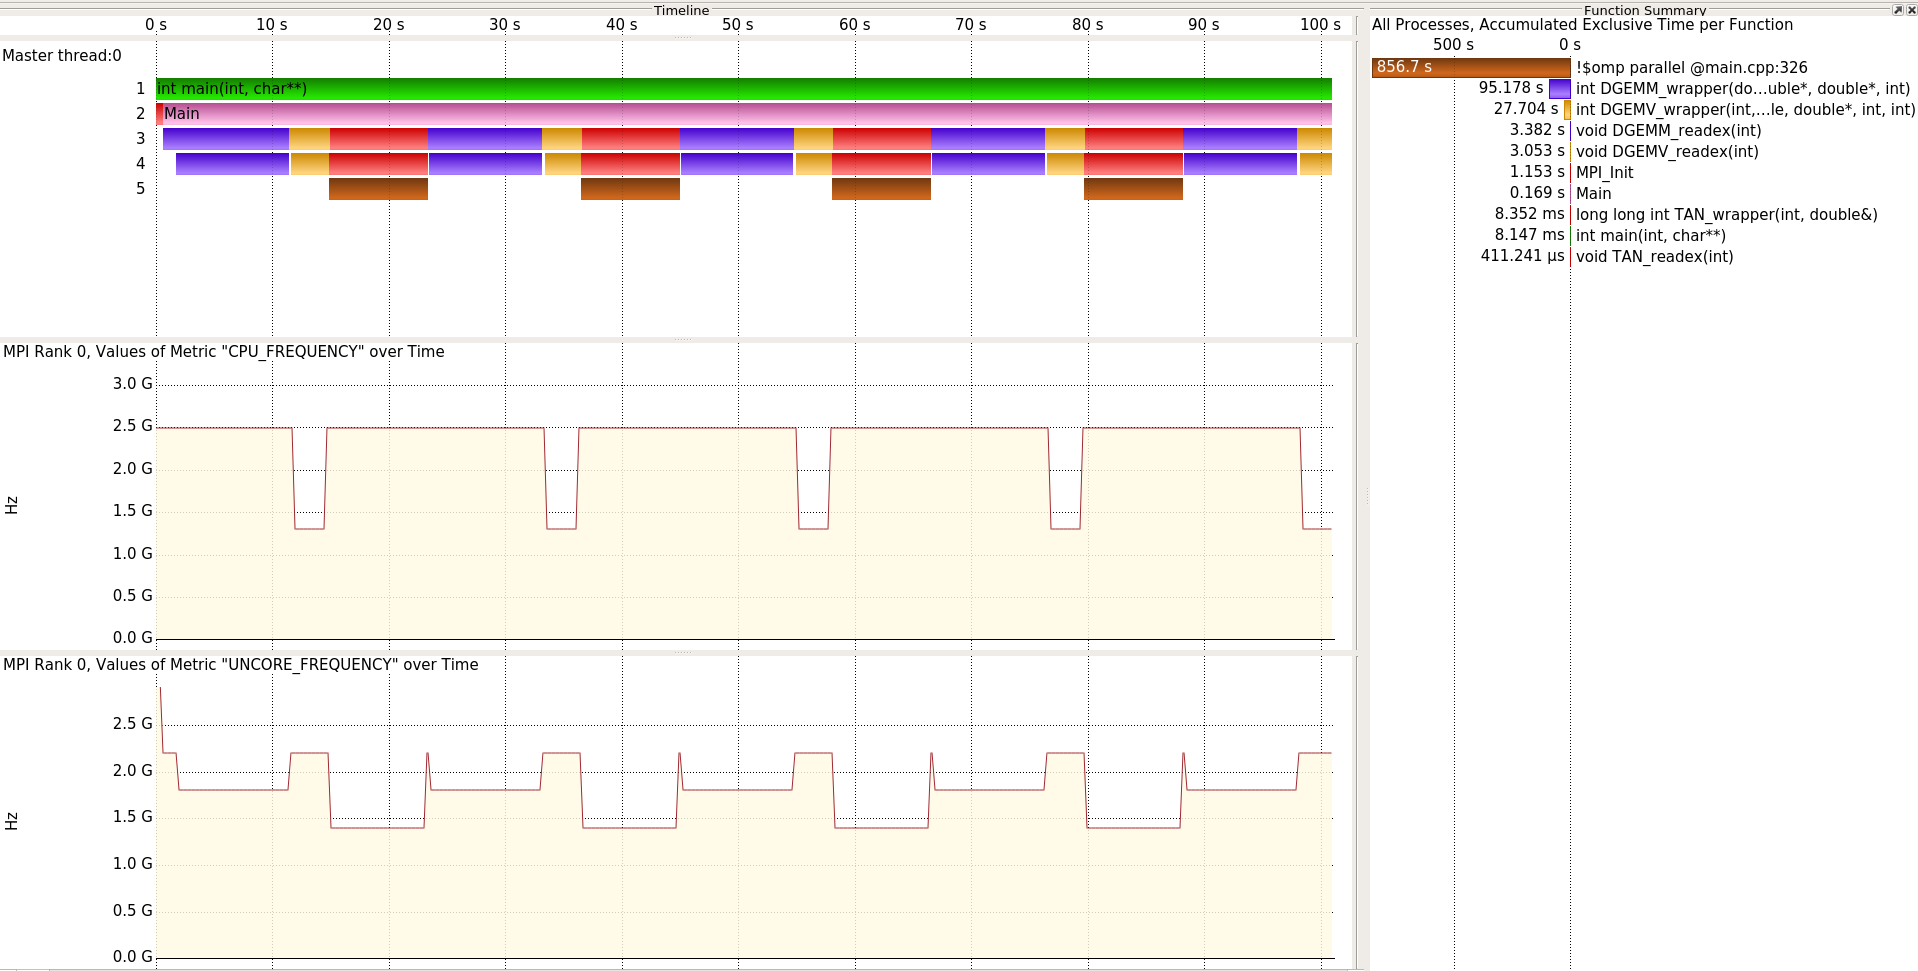
\includegraphics[width=.97\columnwidth]{figures/visualization_trace.png}
	\caption{{CPU\_FREQUENCY} and {UNCORE\_FREQUENCY} switchings during Blasbench runtime tuning}
	\label{fig:switch_visualization}
\end{figure}
 
Figure~\ref{fig:switch_visualization} illustrates the switching of the CPU frequency and uncore frequency tuning parameters performed by RRL while tuning the Blasbench benchmark. The top timeline shows the call stack of the application regions. Below that, we see the CPU frequency changing from 2.5 GHz to 1.3 GHz. Finally, the bottom pane shows the switching of the uncore frequency according to the optimal settings of the different regions.
\newpage

 